\chapter{安裝與基本使用}
雖然現在有強大網頁版的 what you see is what you get 的 
\href{https://www.overleaf.com/}{overleaf},但自己本機裝比較隨心所欲。
有了上面的一些基本觀念,就可以安裝了, 過去有的 distribution 有
\begin{itemize}
 \item teTeX, 古老的 distro ,現在已經被 TeX Live 取代了,就把它想成 slackware 吧。
 \item TeX Live 目前最大的 \TeX distribution。所以我們就裝這個吧。
 \item MacTeX 蘋果用的。
 \item MiKTeX MS-Windows 用的。
\end{itemize}
當然其實在蘋果或MS Windows 也能用 \TeX Live,只是不知道為啥,大家都這樣推薦。
在目前 Linux 環境中,應該還是 \TeX Live 是主流,也簡單。

\section{從 Linux 上安裝}
網路上看很多人說安裝很難,對於 Linux 來說就一行命令就裝完了,真不知道難在哪裡
,真正難在怎麼裝的剛剛好你要的就好。
\\\\
debian/ubuntu
\begin{verbatim}
# apt install texlive-lang-chinese texlive-xetex
\end{verbatim}
redhat/centos/alma/rocky/fedora
\begin{verbatim}
# yum install texlive-collection-langchinese
\end{verbatim}
如果是 CentOS stream, Alma, Rocky 的 distro ,則在AppStream/ repository 下。
\\\\
以 debian / ubuntu 為例。可能碰到的錯誤跟 package
\begin{itemize}
\item texlive-lang-chinese 這個會裝一堆有的沒的包括 Big 5 碼的字型。還有相關
 macro,例如錯誤訊息找不到 ctexhook.sty

\begin{verbatim}
Building PDF for CJK languages fails with 'xeCJK.sty: File `ctexhook.sty' not found
\end{verbatim}

\item texlive-xetex 能處理很多 xetex 的相關 macro,然後奇怪的是 xeCJK 也在這裡。
\item texlive-luatex 能處理很多 luatex 的相關 macro。例如錯誤訊息

\begin{verbatim}
! LaTeX Error: File `luatexbase.sty' not found.
\end{verbatim}

\end{itemize}
裝起來後,debian 裡面的引擎在
\begin{verbatim}
/usr/share/texlive/texmf-dist/tex
\end{verbatim}
下面有
\begin{verbatim}
context  fontinst  generic  latex  latex-dev  
lualatex  luatex  plain  xelatex  xetex
\end{verbatim}
文件在
\begin{verbatim}
/usr/share/doc/texlive-doc
\end{verbatim}
macro 的用法可以在下面找到。使用 distribution 收集的文件閱讀工具 texdoc 來搜尋與閱讀
\begin{verbatim}
$ texdoc -l luatexja
$ texdoc -s ams
\end{verbatim}
不過很多想看的都沒有找到,可能沒有裝 package,所以可能直接 google texdoc amsmath,
texdoc listings 等等的直接幫你找到 CTAN 的文章比較快。新的 
\href{https://texdoc.org}{texdoc 網站}也有搜尋整個 tex 文件的能力。

\section{中文使用}
先來看看我們有什麼字型可以用。fc-list 命令第二欄位就是字型名稱,
可以在 \LaTeX{} 設定中使用的。
\begin{verbatim}
$ fc-list 
\end{verbatim}
grep traditional chinese or taiwan
\begin{scriptsize}
\begin{verbatim}
$ fc-list | grep '\(TC\|TW\)'
$ fc-list :lang=zh-tw
/usr/share/fonts/truetype/arphic/uming.ttc: AR PL UMing TW MBE:style=Light
/usr/share/fonts/opentype/noto/NotoSerifCJK-Bold.ttc: Noto Serif CJK TC:style=Bold
/usr/share/fonts/opentype/noto/NotoSansCJK-Black.ttc: Noto Sans CJK TC,Noto Sans CJK TC Black:style=Black,Regular
/usr/share/fonts/opentype/noto/NotoSansCJK-Regular.ttc: Noto Sans CJK TC:style=Regular
/usr/share/fonts/opentype/noto/NotoSerifCJK-Regular.ttc: Noto Serif CJK TC:style=Regular
/usr/share/fonts/opentype/noto/NotoSerifCJK-ExtraLight.ttc: Noto Serif CJK TC,Noto Serif CJK TC ExtraLight:style=ExtraLight,Regular
/usr/share/fonts/opentype/noto/NotoSansCJK-DemiLight.ttc: Noto Sans CJK TC,Noto Sans CJK TC DemiLight:style=DemiLight,Regular
/usr/share/fonts/opentype/noto/NotoSansCJK-Medium.ttc: Noto Sans CJK TC,Noto Sans CJK TC Medium:style=Medium,Regular
/usr/share/fonts/opentype/noto/NotoSerifCJK-Black.ttc: Noto Serif CJK TC,Noto Serif CJK TC Black:style=Black,Regular
/usr/share/fonts/opentype/noto/NotoSansCJK-Bold.ttc: Noto Sans Mono CJK TC:style=Bold
/usr/share/fonts/opentype/noto/NotoSerifCJK-Medium.ttc: Noto Serif CJK TC,Noto Serif CJK TC Medium:style=Medium,Regular
/usr/share/fonts/truetype/arphic/uming.ttc: AR PL UMing TW:style=Light
/usr/share/fonts/opentype/noto/NotoSerifCJK-SemiBold.ttc: Noto Serif CJK TC,Noto Serif CJK TC SemiBold:style=SemiBold,Regular
/usr/share/fonts/opentype/noto/NotoSansCJK-Regular.ttc: Noto Sans Mono CJK TC:style=Regular
/usr/share/fonts/opentype/noto/NotoSerifCJK-Light.ttc: Noto Serif CJK TC,Noto Serif CJK TC Light:style=Light,Regular
/usr/share/fonts/opentype/noto/NotoSansCJK-Thin.ttc: Noto Sans CJK TC,Noto Sans CJK TC Thin:style=Thin,Regular
/usr/share/fonts/opentype/noto/NotoSansCJK-Bold.ttc: Noto Sans CJK TC:style=Bold
/usr/share/fonts/opentype/noto/NotoSansCJK-Light.ttc: Noto Sans CJK TC,Noto Sans CJK TC Light:style=Light,Regular
\end{verbatim}
\end{scriptsize}
其中第二欄位的名字就是拿來設定字型用的,有逗號表示多種別名。
\\\\
使用古老的 pdftex 引擎也能處理 unicode ,
但選擇能直接處理 unicode ttf/otf 的 lualatex 或 xelatex 引擎與工具。
\\\\
lualatex 範例:

\begin{verbatim}
\documentclass[a4paper,10pt]{book}
\usepackage{luatexja-fontspec}
\setmainjfont{Noto Serif CJK TC}

\begin{document}
\chapter{第一章}
大頭
  \section{第一節}
  小頭
\end{document}
\end{verbatim}

xelatex 範例:

\begin{verbatim}
\documentclass[a4paper,10pt]{book}
\usepackage{xeCJK}
\setCJKmainfont{Noto Serif CJK TC}

\begin{document}
\chapter{第一章}
大頭
  \section{第一節}
  小頭
\end{document}
\end{verbatim}

用標準英文 macro 排點簡單的也可以,
但一些嚴格複雜的排版規矩是會失敗的。

\begin{verbatim}
\documentclass[a4paper,10pt]{book}
\usepackage{fontspec}
\setmainfont{Noto Serif CJK TC}

\begin{document}

\chapter{第一章}
大頭大頭下雨不愁,人家有傘你有大頭。
  \section{第一節}
  小頭銳面難以哉。鄭燮寄弟墨書:「其不發達者,鄉里作惡,小頭銳面,更不可當。」
  頭小而臉尖。形容人刁頑刻薄。又作「小頭小臉」。

\end{document}
\end{verbatim}
lualatex 中文社群決定不開發新的 package ,沿用日本的 luatexja 就好,因為
漢字處理兩者是一樣的,即使 CJKV 這四個漢字圈的韓國越南大概也不用漢字了。
\\\\
命令差別在於設定字型新命令,setmainjfont, setCJKmainfont, 與標準英文的
setmainfont。之所以要使用特別 package 在於排版規矩,漢字與英文在斷行,
間隔,空白,寬度計算上有些不同,又或者漢字能直排等等。如果不是很在意排
版效果,用全英文的命令都可以。
\\\\
命令產生 pdf 檔

\begin{verbatim}
$ xelatex test.tex
$ lualtex test.tex
\end{verbatim}

如果有錯誤發生,應該是某相依 macro 沒有裝起來,去 google 看要裝什麼名字,
在系統中安裝。過去可能會先產生 dvi 檔,再由 dvi 轉成各種輸出,或者將 latex 
轉成 html, opendoc 等等,不過現在網路速度很快,使用 pdf 在線閱讀也沒問題,
所以也不再做這些輸出,有興趣的就自己玩其他的工具。
\\\\
有的例子會用 \verb=\usepackage{CJK}= 套件,這個套件是舊的 pdftex 使用的,
所以它的目錄編排方式好像還是以前 teTeX 的 /usr/share/texmf/tex 而不是
/usr/share/texlive/texmf-dist, 它也有 UTF8 編碼, 如果真有 Big5, 
GB, JIS 編碼舊文件要處理,也可以用這套件,只是 pdftex 它字型使用
必須是相關 tfm/map 已經建立,所以若是建立不完全則無法使用。
而設定名字必須是從 fd 檔裡面找到真正字型名稱用在 CJK package 裡面。
我就是從 /usr/share/texlive 跟 /usr/share/texmf 下面搜尋 fd 檔,
然後去看名稱,因此用 pdflatex 除非自己懂造新字型的,不然是很受限
於 distro 給你的字型。
\\\\
pdflatex 範例
\begin{verbatim}
\documentclass[a4paper,10pt]{book}
\usepackage{CJK}

\begin{document}
\begin{CJK}{UTF8}{bkai}
\chapter{第一章}
大頭大頭下雨不愁,人家有傘你有大頭。
  \section{第一節}
  小頭銳面難以哉。鄭燮寄弟墨書:「其不發達者,鄉里作惡,小頭銳面,更不可當。」
  頭小而臉尖。形容人刁頑刻薄。又作「小頭小臉」。

\end{CJK}
\end{document}
\end{verbatim}
使用命令為 
\begin{verbatim}
$ pdflatex test.tex
\end{verbatim}
這個 bkai 名字是 fd 檔案裡面的,這是 Big 5 楷書,只是用 pdflatex 引擎,
可以轉換 Big 5 到 UTF8。 最後編譯如果出錯,都會有個 xxx.log 檔,裡面會有
整個編譯總結,錯誤訊息都在裡面。

\section{進階安裝}
其實像我安裝 Linux 時,我都是裝我需要的東西就好,有些大 package 的安裝,
裝了一大堆亂七八糟的東西,但要做到只安裝有需要的,就必須對整個系統有粗淺的了
解才有可能。
\\\\
texlive 最基本會包 plain \TeX, pdftex, luatex
\subsection{最小安裝 - deb package}
從目前 debian/ubuntu 的 package 來看
\begin{itemize}
\item texlive-base 只有包含引擎 tex, pdftex, luatex
\item texlive-binaries dvi, metafont, metapost, ps 等處理程式,然後還有 xetex。
\item texlive-latex-base 包含 latex, pdflatex, lualatex
\item texlive-xetex 才會包含 xelatex 與相關工具。
\item texlive-luatex 才會包含相關 macro 。
\end{itemize}
不知道為什麼目前 xetex 是被特別對待的,也就是 luatex 是自動在 texlive-base,
但 xetex 卻是在 texlive-binaries,總之,base 與 binaries 是引擎與基本工具。
\\\\
中日韓套件
\begin{itemize}
\item texlive-lang-xxxx 這些才是新的 \XeTeX 需要的。
  \begin{itemize}
  \item texlive-lang-chinese 是真正有一些中文處理 sty ,fd 檔,與文鼎
   truetype 字型,會把 texlive-lang-cjk 這些亂七八糟的全裝起來。
   這些 package 實在分類裝的亂七八糟的。
  \item texlive-lang-cjk 一些 mapping 檔。
  \item texlive-xetex 裡面才有真正 xeCJK macro
  \end{itemize}
\item latex-cjk-xxxx 都是舊的古老的工具
  \begin{itemize}
  \item latex-cjk-chinese 是真正有如 bg5latex,包含big5, gb 碼等工具。
        如果改用新的 unicode {\XeTeX} luatex 引擎,這些是可以不要裝的。
  \item latex-cjk-common 是用在 pdftex 上的 macro
  \end{itemize}
\end{itemize}
字型在以前是系統跟 \TeX 系統是分開的,要分別為他們兩個需求建立特別系統需要檔案,
現在 {\XeTeX} luatex 能統一用所有的,系統上就應該是免費的 google No Tofu 
計畫裡面的 opentype ,同樣 latex-cjk-xxx 的是舊的特有 \TeX 需求檔案,font-xxx
是系統字型檔。
\begin{itemize}
\item fonts-noto-cjk google 的開源 No Tofu 思源字體。系統上 opentype 字體。
\item fonts-arphic-xxx 文鼎 truetype 字型,有人改了原本type1 big5 編碼成為 
truetype unicode 編碼給大家用。
\item fonts-wqy-xxx 文泉驛字型。
\item latex-cjk-chinese-arphic-xxx 這是舊的文鼎 type 1 字型。
有 tfm, fd 與 pfb 檔建好了,所以以前都是用這個。這還是可以給 xetex/luatex
繼續用,只不過字型命名方式不一樣。
\end{itemize}
pdftex 引擎比較麻煩,在 TEXMFHOME 目錄下搜尋 fd 檔,字型名字在裡面
,TEXMFHOME 應該在 /usr/share/texlive 與 /usr/share/texmf。
\\\\
所以真正安裝
\begin{itemize}
\item xelatex 這要裝 texlive-xetex, texlive-lang-chinese,
但它的 dependancy 太多。
\item lualatex 這要裝 texlive-luatex
\item fonts 喜歡的裝就好了。
\end{itemize}
rpm 形式的反而比 deb 的複雜很多。就先不管它了

\subsection{最小安裝 - 從CTAN}
如果沒有 root 權限,或不想裝 Linux 系統 package ,那麼就自己從 CTAN 抓 texlive
來,只是這我裝起來也要1G,也蠻大的。
\begin{enumerate}
\item \href {http://mirror.ctan.org/systems/texlive/tlnet/install-tl-unx.tar.gz}{CTAN 下載}
\item 執行 ./install-tl
\item 調整選項,按 S 選 c ,small scheme, 這個會裝 xetex 引擎。
\item 繼續調整其他,按 D 像是 TEXDIR TEXMFHOME 目錄。
\item 裝完後,要多增加 PATH, MANPATH, INFOPATH,就可以用了。
\end{enumerate}
\begin{center}
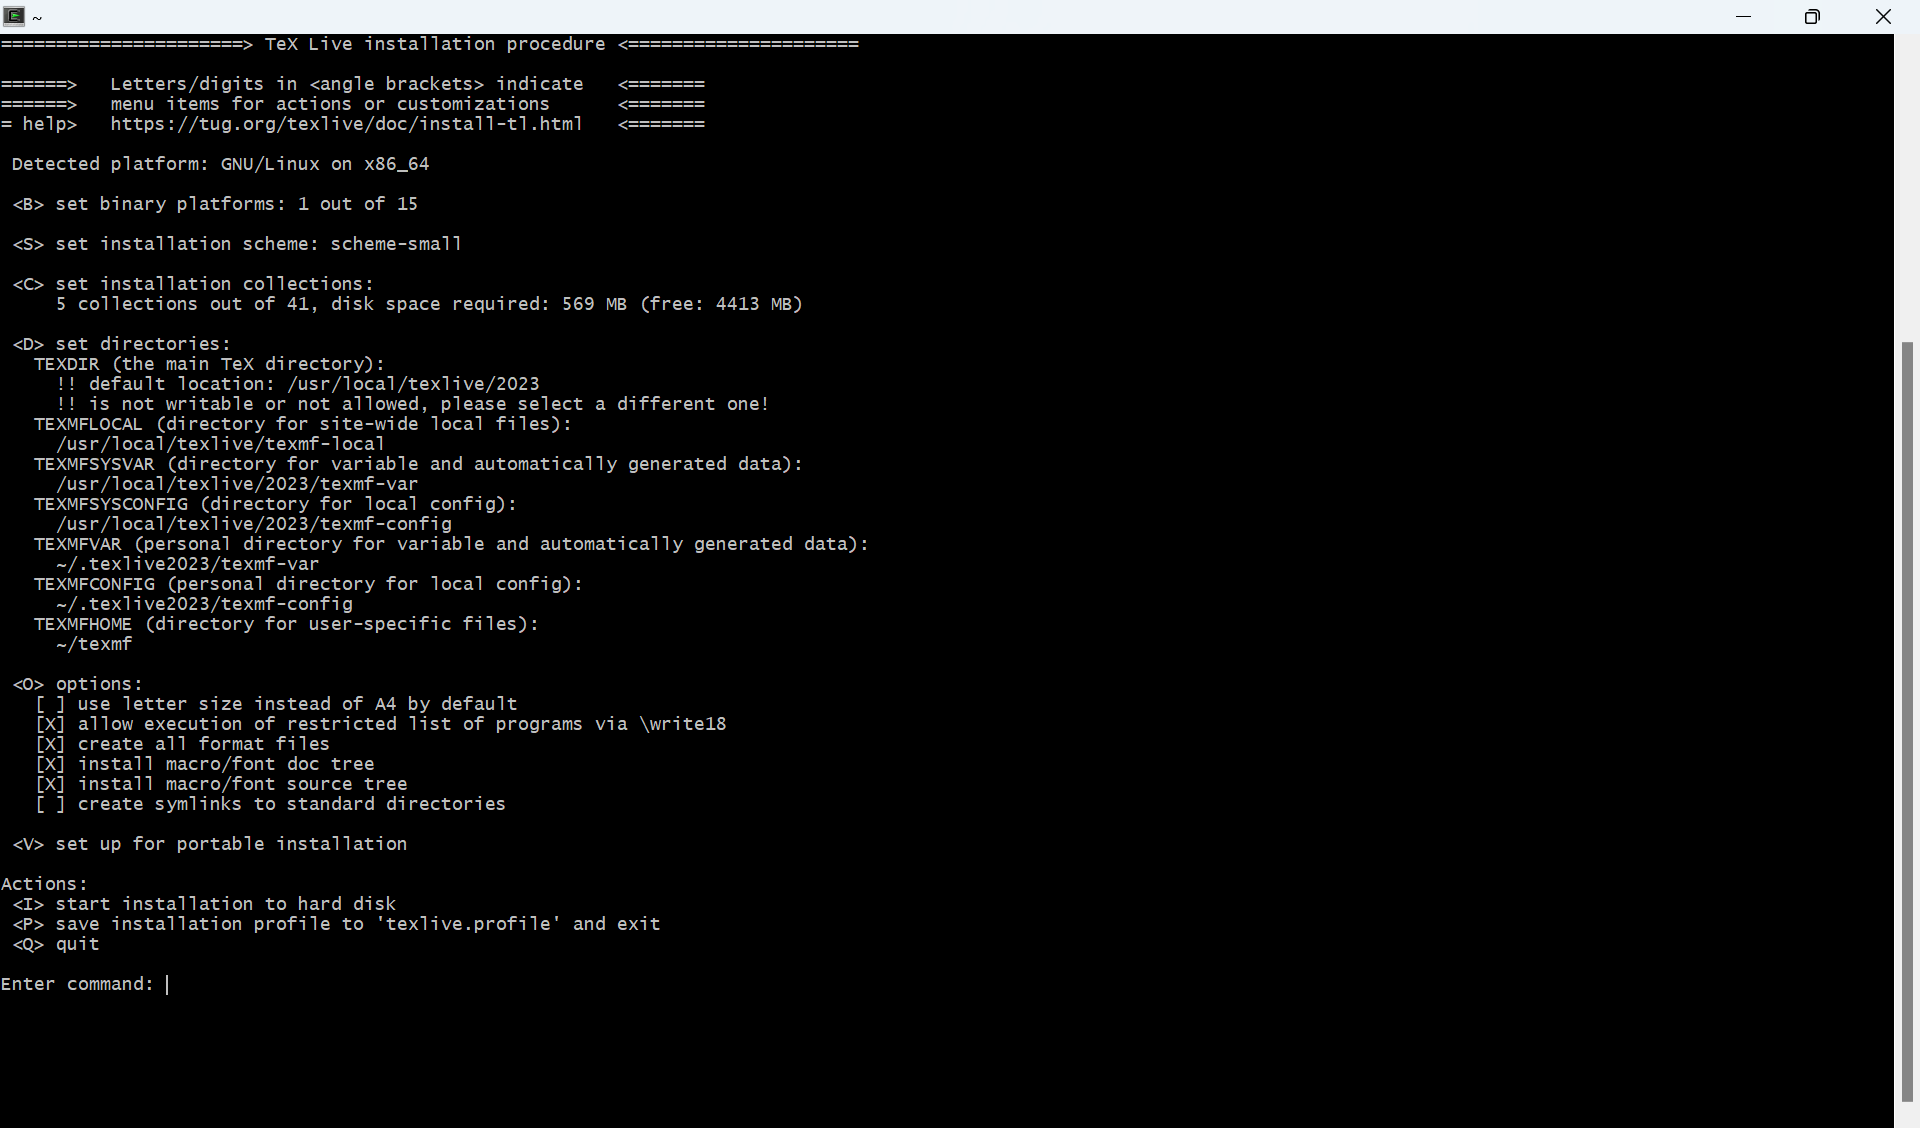
\includegraphics[width=\textwidth,height=0.6\textwidth]{images/texlive.png}
\end{center}
試看看最基本的命令
\begin{verbatim}
$ tex '\empty Hello world!\bye'
$ pdftex '\empty Hello world!\bye'
\end{verbatim}
像 python 用 pip ,perl 用 cpan,texlive 也有工具來管理 package,
而且也是遠端跟 CTAN 直接溝通的管理, 使用 tlmgr 來管理 macro。
package 管理只有幾件重要事情
\begin{itemize}
\item 遠端 repository 是誰?內定是 CTAN。
\item 本地端要裝在哪裡? 這應該在 TEXDIR 下。
\item 現在裝了什麼?
\item 如何安裝新的與移除不要的?
\item package 資訊與 package 裡面有什麼檔案?
\item 如何升級?
\item 怎麼移除全部安裝?
\end{itemize}
看看裝了什麼 package
\begin{verbatim}
$ tlmgr list
\end{verbatim}
安裝移除。我們是要裝 xecjk 的,所以 remove 只是命令。
\begin{verbatim}
$ tlmgr install xecjk
$ tlmgr remove xecjk
\end{verbatim}
package 的資訊
\begin{verbatim}
$ tlmgr info xecjk
$ tlmgr info --list xecjk
\end{verbatim}
尋找
\begin{verbatim}
$ tlmgr search --global --file cfr-lm.sty
$ tlmgr list | grep ducks 用 search 有的是找不到,用 grep 比較好
\end{verbatim}
升級
\begin{verbatim}
$ tlmgr update --list
$ tlmgr update --all
\end{verbatim}
設定原本的內定值,例如換掉遠端 repository 的位址
\begin{verbatim}
$ tlmgr option repsoitory https://mirror.ctan.org/systems/texlive/tlnet
$ tlmgr paper letter
\end{verbatim}
不爽玩了,整個毀掉
\begin{verbatim}
$ tlmgr uninstall
\end{verbatim}

\subsection{字型}
除了 Linux package 上有的,也可自行去抓 ttf 或者 otf 檔。如果沒有權限裝在系統
上,可以下載到 
\begin{verbatim}
$HOME/.local/share/fonts 
或者舊的
$HOME/.fonts 下
\end{verbatim}
然後用
\begin{verbatim}
$ mkfontscale
$ mkfontdir
$ fc-list
\end{verbatim}
製作向量字型 index 。
\\\\
下載中文字型,不過這很多在系統 package 上也是有啦,現在主要用 google
Adobe 合作的 opensource 思源字體,Noto 字體,不過用系統裝的跟下載的名字
有時會不同,不知為啥,我用 debian 系統package裝的是
Noto Sans CJK TC 但自己下載的變成 Noto Sans TC,所以這個名字要自己根據
fc-list 看到得來。不過台灣官方的全字庫跟教育部標準應該蒐集字是最齊全的,有些
冷門字,或許他們才有。
\begin{enumerate}
\item \href{https://data.gov.tw/dataset/5961}{數位發展部的全字庫宋體與楷書}
\item \href{https://language.moe.gov.tw/result.aspx?classify_sn=23&subclassify_sn=436}{教育部國字標準字體-宋楷隸}
\item \href{https://source.typekit.com/source-han-serif}{Adobe 的開源opentype思源字型}
\item \href{https://fonts.google.com/}{Google 的思源字體下載}
\item \href{https://github.com/fontworks-fonts}{日本Fontworks Inc的七款日文字體}
\item \href{https://github.com/googlefonts/kosugi-maru}{日本-日文小杉丸體}
\item \href{https://github.com/ichitenfont/I.Ming}{一點明體-修改日本 ichiten 的明體}
\item \href{https://sites.google.com/view/jtfoundry/zh-tw}{台北黑體-翰字鑄造公司改造思源適合印刷字型}
\item \href{https://github.com/ButTaiwan/iansui}{芫荽字體-新增改造fontworks 的klee而來}
\item \href{https://github.com/justfont/open-huninn-font}{粉圓體-新增改造小杉丸來}
\item \href{https://github.com/l10n-tw/cwtex-q-fonts}{cwTeX truetype}
\item \href{https://code.google.com/archive/p/wangfonts/}{王漢宗老師的48套字型}
\end{enumerate}
由於xelatex 是走系統字型, 系統字型套件是 fontconfig, 字型放在 /usr/share/fonts
\$HOME/.local/share/fonts 或者 \$HOME/.fonts ,設定在 /etc/fonts,
/usr/share/fontconfig,\$HOME/.config/fontconfig \$HOME/.fontconfig 下的
fonts.conf 與裡面的 conf.d 目 錄。 所以如果是手動用 install-tl 裝 texlive 的,
那要把 texlive 字型告訴 fc 進到系統字型設定中。 在安裝目錄下的
\begin{verbatim}
./texmf-var/fonts/conf/texlive-fontconfig.conf
\end{verbatim}
已經有 texlive 給 fontconfig 用的 conf 檔,是根據當初給的 TEXDIR TEXMFHOME
目錄建立的。因此只要 symlink 這檔案到
\begin{verbatim}
/etc/fonts/conf.d/90-texlive-fontconfig.conf
或
~/.config/fontconfig/confd.d/90-texlive-fontconfig.conf
或
~/.fonts.conf.d/90-texlive-fontconfig.conf
\end{verbatim}
就可以 fc-list 看到他們,
\\\\
texlive 在他目錄下 texmf-dist/fonts/type1 裡面 cjk 帶有 arphic 繁體字字型,
是文鼎以前 open 的字型,texmf-dist/fonts/misc/cns 裡面有 CNS 國家中央標準局
的 bitmap 字型,這好像是現在數位發展部負責了。但 arphic 是 Big5,而 cns 是
CNS 碼還是 bitmap,所以我想應該沒人會用了,不知道為啥安裝 cjk 套件還裝這些。
當用
\begin{verbatim}
tlmgr list | grep arphic
\end{verbatim}
還會發現有 arphic-ttf ,但也是 Big 5 的。 如果沒有抓其他的字體,光想用
texlive 原裝內定的下載使用 unicode 正體中文,
\begin{itemize}
  \item 使用傳統 pdflatex 用 \verb=\usepackage{CJK}= 與
    \verb=begin{CJK}{UTF8}{bkai}=
  \item 要不就是檔案是 input Big 5 使用 xelatex,lualatex 的 arphic-ttf
  \item fontspec 會自己抓 input encode (character code set) 跟 font encode 
    (font code set) 但這個要有 def 檔定義,目前好像沒有 big5<->utf8 定義檔
    給 xelatex 用。
  \item 自己用arphic Big5 生成 arphic unicode ttf/otf,不過這對新手有點煩。
    這乾脆下載自己的ttf 還比較快。debian 裡面有 arphic utf8 的 ttf package
    但這已經不是 texlive 原裝的了。
\end{itemize}
type1 基本上已經很老舊,對新手不是很好用,只是不知道為啥 Texlive 裡面
有中國大陸的 fando 簡體中文字型, 沒有 unicode 正體中文 ttf/otf,
連 noto 中文 TC 字型也沒有收錄。
